\section{True RMS jaudas detektora un RF kabeļu tests}
S-parametru noteikšanai tiek veikti no 6.5 līdz 8.5 GHz diapozonā. Tiek veikts koaksiālo kabeļu RFC1 un RFC2 S-parametru (skat. att. 2.1.), kas savieno atzarotāja $P_{fwd}$ un $P_{ref}$ ar jaudas detektoru un jaudas detektora novērtējums. Tad jaudas detektora izejas sprieguma atkarība no ieejas signāla jaudas pie 7.2 GHz.
\begin{figure}[H]
	\centering
    \includegraphics[width=0.7\textwidth]{pictures/cable_coax_fwd.jpg}\hspace{1cm}
    \caption{Izstarotās jaudas koaksiālais kabeļa S-parametri}
\end{figure}
Lielākā daļa no ienākošās jaudas koaksiālajā kabelī netiek atstarota ($S_{11}$ un $S_{22}$) atpakaļ -24 dB, kas ir aptuveni 0.4\% no jaudas, bet, neskatoties uz to, pašā vadā ir -1.8 dB zudums ($S_{21}$ un $S_{12}$), kas ir aptuveni 33\% no ienākošās jaudas.
\begin{figure}[H]
	\centering
    \includegraphics[width=0.7\textwidth]{pictures/cable_coax_ref.jpg}\hspace{1cm}
    \caption{Atstarotās jaudas koaksiālais kabelā S-parametri}
\end{figure}
Lielākā daļa no ienākošās jaudas koaksiālajā kabelī netiek atstarota ($S_{11}$ un $S_{22}$) atpakaļ -20 dB, kas ir aptuveni 1\% no jaudas, bet, neskatoties uz to, pašā kabelī ir -1.9 dB zudums ($S_{21}$ un $S_{12}$), kas ir aptuveni 36\% no ienākošās jaudas.
\begin{figure}[H]
	\centering
    \includegraphics[width=0.7\textwidth]{pictures/tests_diagram3.png}\hspace{1cm}
    \caption{Jaudas detektora testu diagramma}
\end{figure}
3.14. att. redzams testa iekārtu slēgums elektriski principiālajā shēmā.
\begin{figure}[H]
	\centering
    \includegraphics[width=0.7\textwidth]{pictures/vna_measurement_powerdet.jpeg}\hspace{1cm}
    \caption{S-parametri jaudas detektoram}
\end{figure}
Izstarotā un atstarotā jaudas kanāli atstaro aptuveni pusi no ienākošā signāla jaudas. Savstarpējā portu izolācija ir laba, kas tiek panākta ar metalizētiem urbumiem.
\begin{figure}[H]
\centering
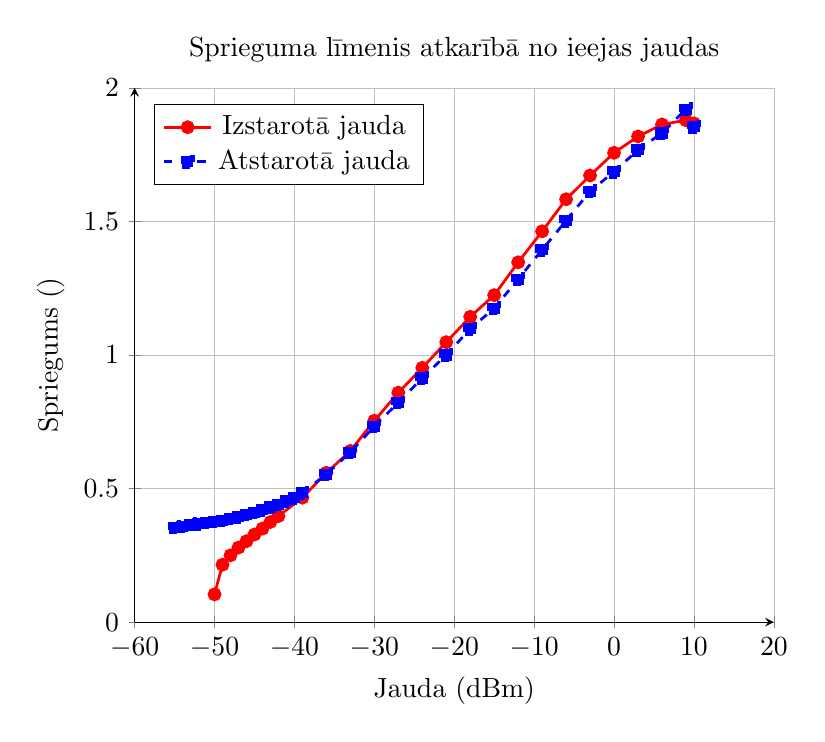
\begin{tikzpicture}
\begin{axis}[
    title={Sprieguma līmenis atkarībā no ieejas jaudas},
    xlabel={Jauda (dBm) },
    ylabel={Spriegums (\si{\volt})},
    xmin=-60, xmax=20,
    ymin=0, ymax=2,
    grid=both,
    grid style={line width=0.1pt, draw=gray!50},
    width=0.8\textwidth,
    axis lines=left,
    legend pos=north west,
]

% Line 1: FWD power (Red)
\addplot[
    color=red,
    mark=*,
    line width=1pt,
]
coordinates {
    (-50, 0.104)
    (-49, 0.215)
    (-48, 0.250)
    (-47, 0.279)
    (-46, 0.303)
    (-45, 0.328)
    (-44, 0.350)
    (-43, 0.375)
    (-42, 0.397)
    (-39, 0.466)
    (-36, 0.559)
    (-33, 0.641)
    (-30, 0.754)
    (-27, 0.859)
    (-24, 0.952)
    (-21, 1.048)
    (-18, 1.143)
    (-15, 1.224)
    (-12, 1.347)
    (-9, 1.463)
    (-6, 1.583)
    (-3, 1.672)
    (0, 1.757)
    (3, 1.818)
    (6, 1.863)
    (9, 1.879)
    (10, 1.867)
};
\addlegendentry{Izstarotā jauda}

% Line 2: REF power (Blue)
\addplot[
    color=blue,
    mark=square*,
    dashed,
    line width=1pt,
]
coordinates {
    (-55, 0.355)
    (-54, 0.358)
    (-53, 0.366)
    (-52, 0.368)
    (-51, 0.373)
    (-50, 0.377)
    (-49, 0.382)
    (-48, 0.388)
    (-47, 0.394)
    (-46, 0.403)
    (-45, 0.412)
    (-44, 0.420)
    (-43, 0.431)
    (-42, 0.442)
    (-41, 0.454)
    (-40, 0.466)
    (-39, 0.484)
    (-36, 0.554)
    (-33, 0.636)
    (-30, 0.733)
    (-27, 0.822)
    (-24, 0.914)
    (-21, 1.000)
    (-18, 1.098)
    (-15, 1.175)
    (-12, 1.284)
    (-9, 1.394)
    (-6, 1.503)
    (-3, 1.613)
    (0, 1.686)
    (3, 1.768)
    (6, 1.831)
    (9, 1.920)
    (10, 1.855)
};
\addlegendentry{Atstarotā jauda}

\end{axis}
\end{tikzpicture}
\caption{Izejas sprieguma ietekme uz ieejas jaudu}
\end{figure}
Iegūstot izejas sprieguma līmeņu atkarības no ieejas jaudas, tika ņemti vērā signāla ģeneratora un vada zudumi. Līkne, kas tika iegūta abos kanālos, ir ļoti līdzīga ražotāja dotajai specifikācijai. Jutības diapazons ir no -50 līdz 9 dBm, kur 0 dBm atbilst 100 W, tad mēs varam izmērīt no 1 mW līdz 794,3 W.